\subsection{Logical view}\label{ssec:planlaegning:logicalview}
Dette afsnit skal forklare applikationslogikken for plannings i webapplikationen.
\\ \\
Bussiness logikken vil blive lagt i en controller, for at overholde MVC strukturen. Dertil vil PlanningControlleren komme til at stå for at håndtere brugers anmodninger og render views med modeldata. Til udarbejdelsen af arkitekturen for PlanningControlleren er der lagt vægt på US's, hvor der er arbejdet agilt med dokumentationen samt implementeringen. Dertil er ikke alle US implementeret endnu, men vil blive i fremtidige iterationer. \\

\noindent Ud fra arkitekturen beskrevet i bilag \cite{ArkitekturPlanning}, så er et klassediagram udarbejdet, som der kan tages udgangspunkt i til design og implementeringen. Klassediagrmmet ses nedenfor på figur \ref{fig:ark_planning_logic_classdiagram}.

\begin{figure}[H]
  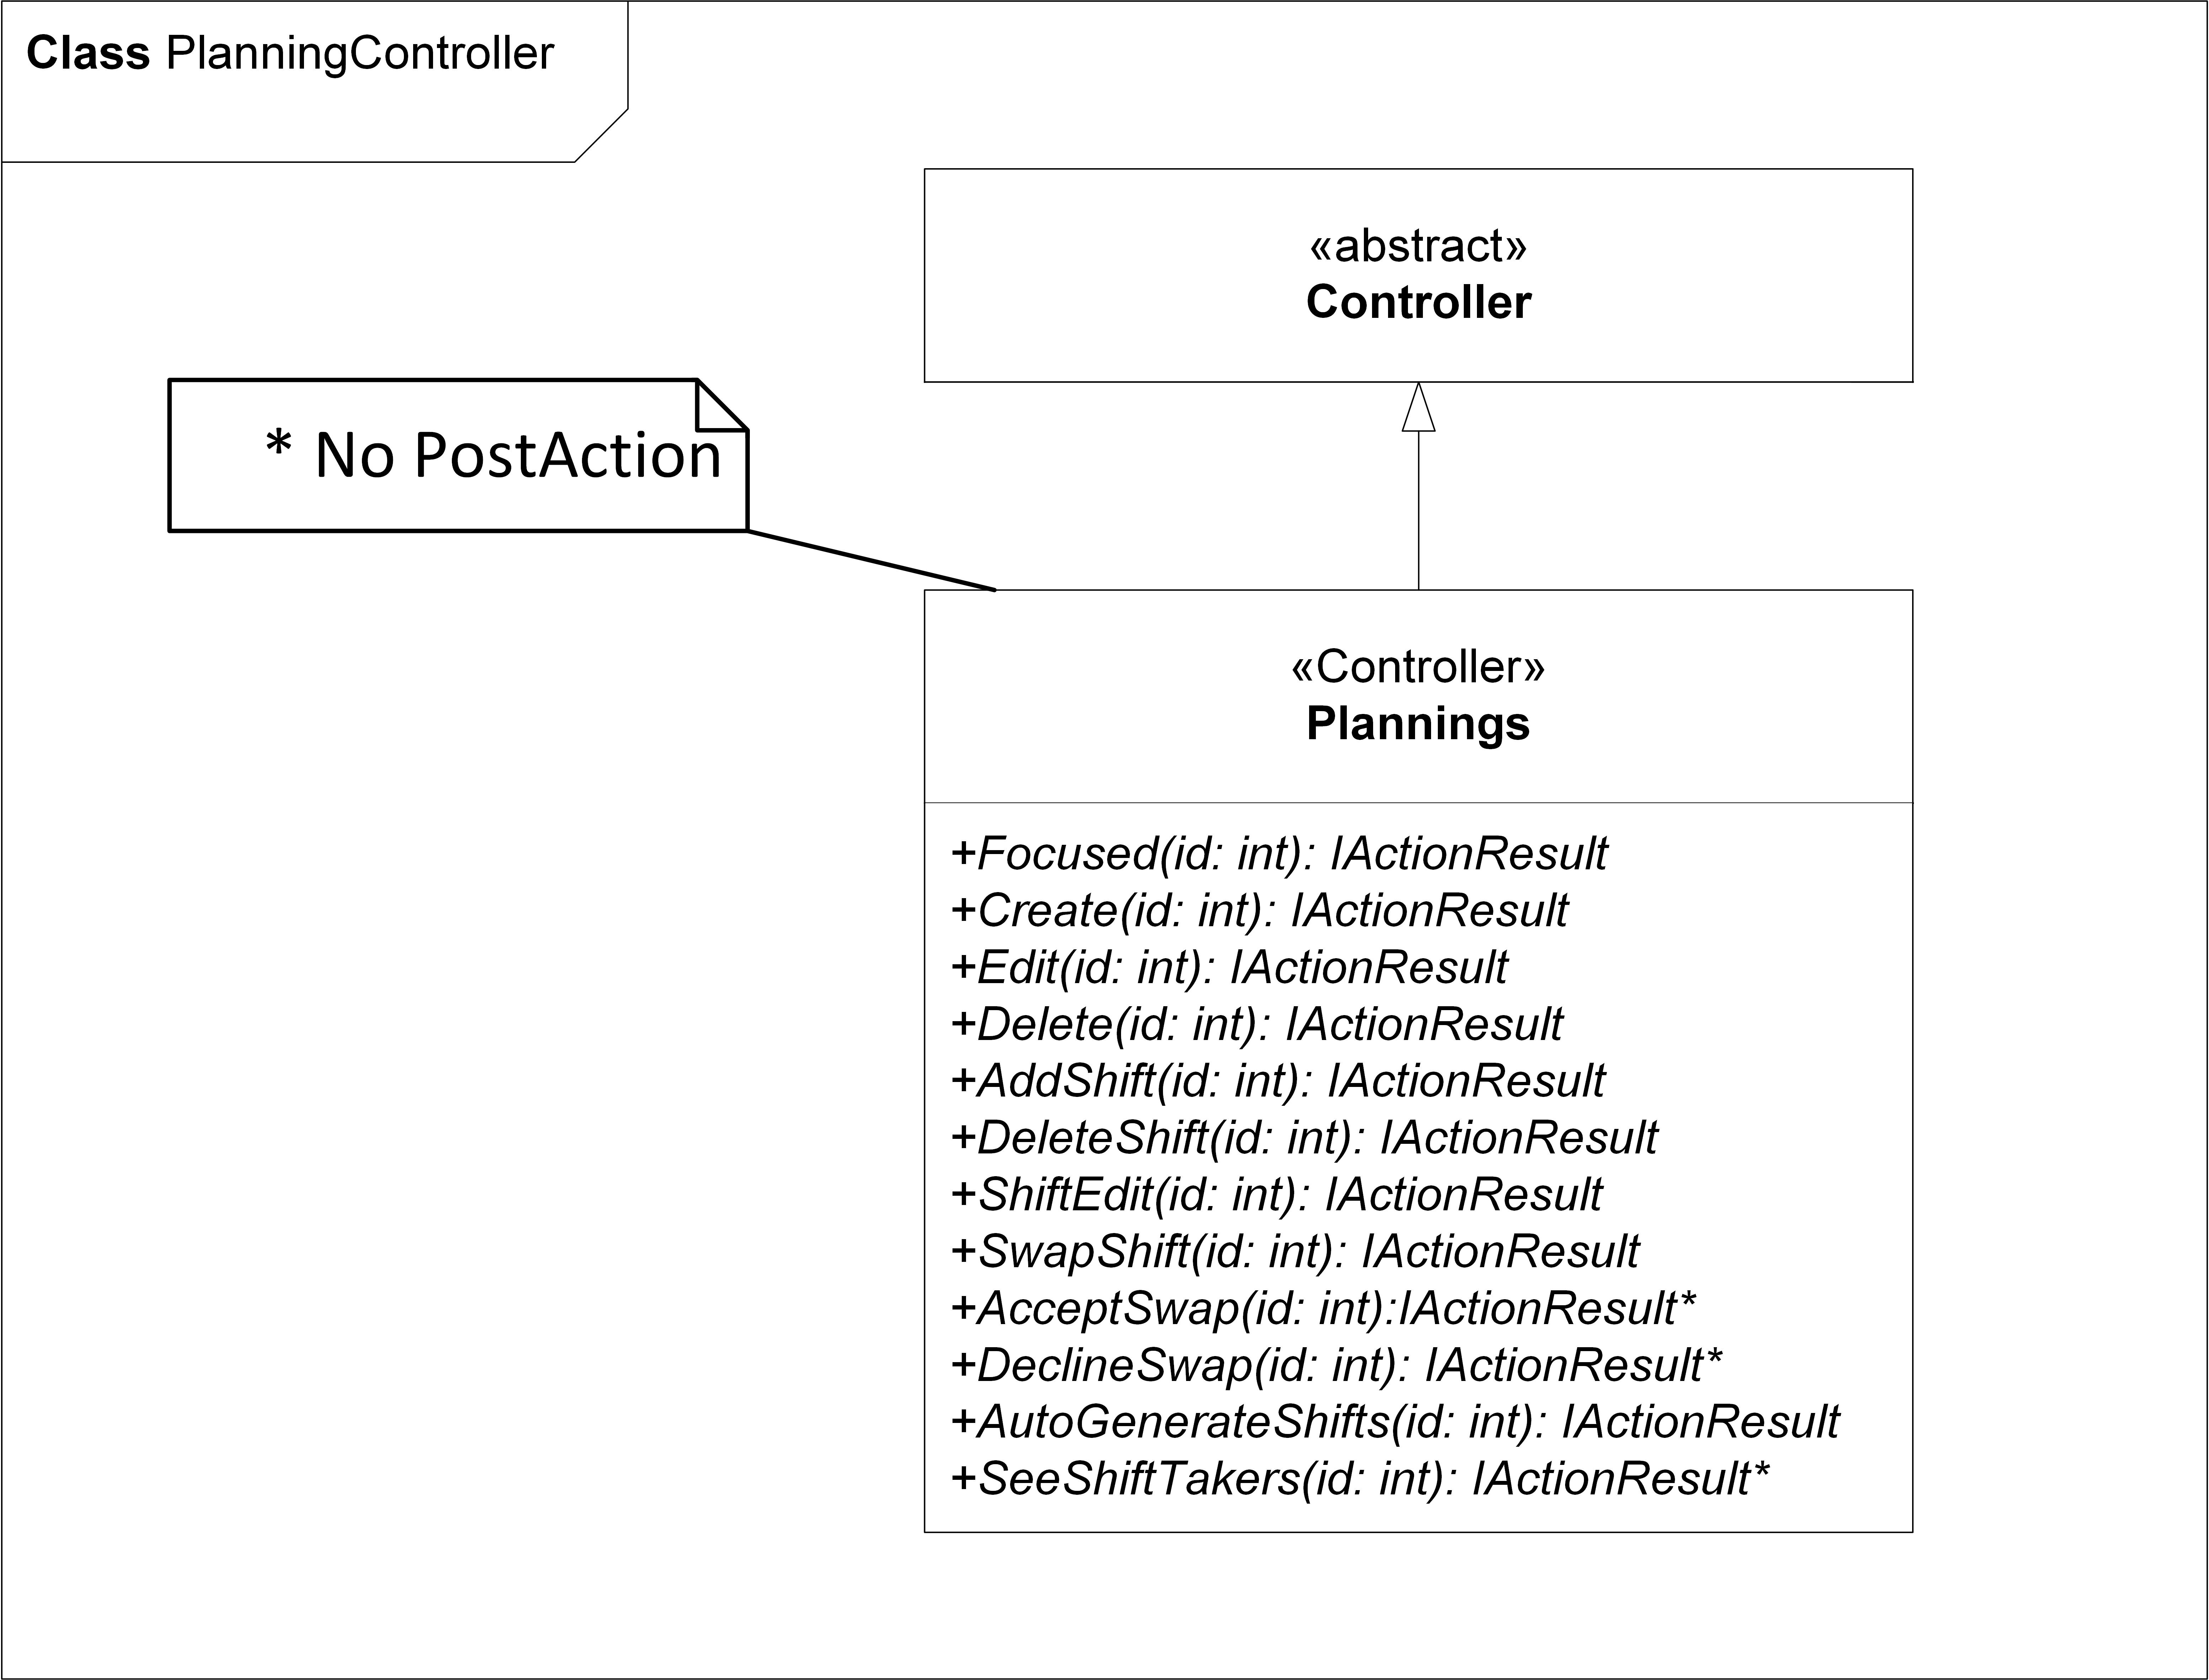
\includegraphics[scale=0.8]{09_Arkitektur/Planning/pictures/CD_Planning.jpg}
  \centering
  \caption{Klassediagram for planningController med de nødvendige metoder til at gennemføre de valgte US}
  \label{fig:ark_planning_logic_classdiagram}
\end{figure}

